\chapter{Realizacja projektu}
%_______________________________________________________________________________________________________________
\section{Część sprzętowa}
\subsection{Przerzutka }
 Zasada działania serwomechanizmu kontrolującego pozycję wózka została przedstawina na rys. \ref{fig:przerzutkaSerwo}. Zmiana pozycji wału serwomechazmu implikuje zmianę pozycji wózka poprzez zastosowanie sztywnego połączenia przegłubowego.
 \begin{figure}[h]
    \centering
    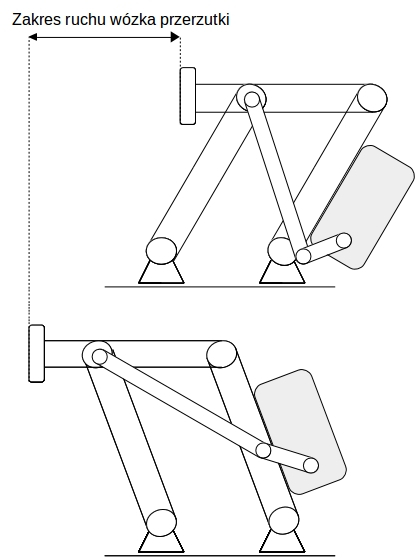
\includegraphics[scale=0.5]{przerzutkaSerwo.jpg}
    \caption{Zasada działania przerzutki rowerowej z wykorzystaniem serwomechanizmu}
    \label{fig:przerzutkaSerwo}
\end{figure}

Przymocowanie serwomechanizmu do przerzutki, zgodnie ze schematem przedstawionym na rys. \ref{fig:przerzutkaSerwo}  można podzielić na kilka etapów.
Pierwszy etap to usunięcie sprężyny, która występuje w konwencjonalnych przerzutkach tylnych. Wiąże się to ze zniszczeniem połączeń nitowych do których przymocowana jest sprężyna. Zniszczone połączenia nitowe zastąpione zostały przez połączenia śrubowe. Wykorzystane zostały śruby z gwintem metrycznym M4 o średnicy 4 mm.

Następny etap to wykonanie elementu mocującego serwomechanizm do przerzutki. Element został wykonany zgodnie z projektem przedstawionym na rysunku technicznym \ref{fig:lacznik}.
\begin{figure}[h]
    \centering
    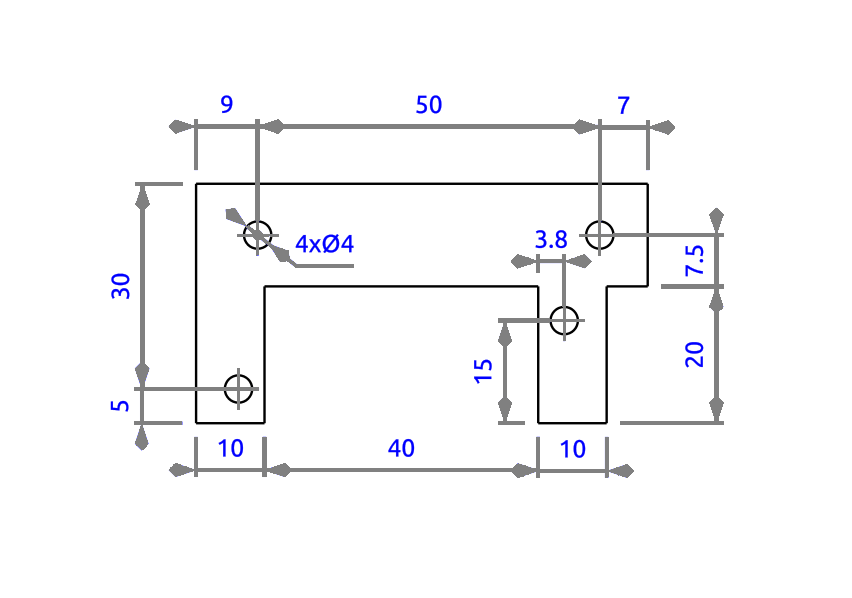
\includegraphics[scale=0.4]{lacznik.png}
    \caption{Schemat ilustrujący zasadę działania programu kontrolera}
    \label{fig:lacznik}
\end{figure}

Wykonany element wraz z połączeniami śrubowymi umożliwa przymocowanie serwomechanizmu Hitec Hs-8335SH do przerzutki SRAM X5. Ostatni etap tej części projektu to wykonanie połączenia przegłubowego łączącego wał serwomechanizmu z jednym z członów ruchomych przerzutki. Autor zdecydwał się na zastosowanie modelarskiego drążka kierwoniczego o zmiennej długości oraz dedykowanego aluminowego orczyka serwomechanizmu. Takie rozwiązanie pozwala dokładnie dopasować długość  połączenia, bez konieczności projektowania oraz wykonania dodatkowych elementów.

W wyniku poywższych czynności powstała w pełni funkcjonalna przerzutka tylna sterowana przy użyciu serwomechanizmu. 

%_______________________________________________________________________________________________________________
\subsection{Integracja elementow elektronicznych}
Miktrokontroler, filtry RC, pakiet zasilający, regulator napięcia oraz jednostka pomiarowa IMU zamontowane zostały w hermetycznej puszcze elektrycznej, przymocowanej na stałe do dolnej rury przedniego trójkąta ramy rowerowej. 

Schemat połączeń znajduje się na rys. \ref{fig:schematPolaczen}. Na schematcie przedstawione zostały jedynie elementy wykoanne przez Autora pracy. Są to filtry RC, dzielnik napięcia do pomiaru stanu pakietu zasilającego, połączenia do sterowania serwomechanizmem oraz połączenia do komunikacji z jednostką pomiarową IMU. Szczegóły związane z dystrybucją zasilania zostały pominięte, ponieważ są elementem zestawu uruchomieniowego. Można je znaleźć w \textcolor{red}{tivaWorkBook}. Ze względu na rozwojowy charakter projektu oraz częste zmiany wprowadzane na etapie realizacji, autor pracy nie zdecydował się na wykonanie dedykowanego obwodu drukowanego.
\begin{figure}[h]
    \centering
    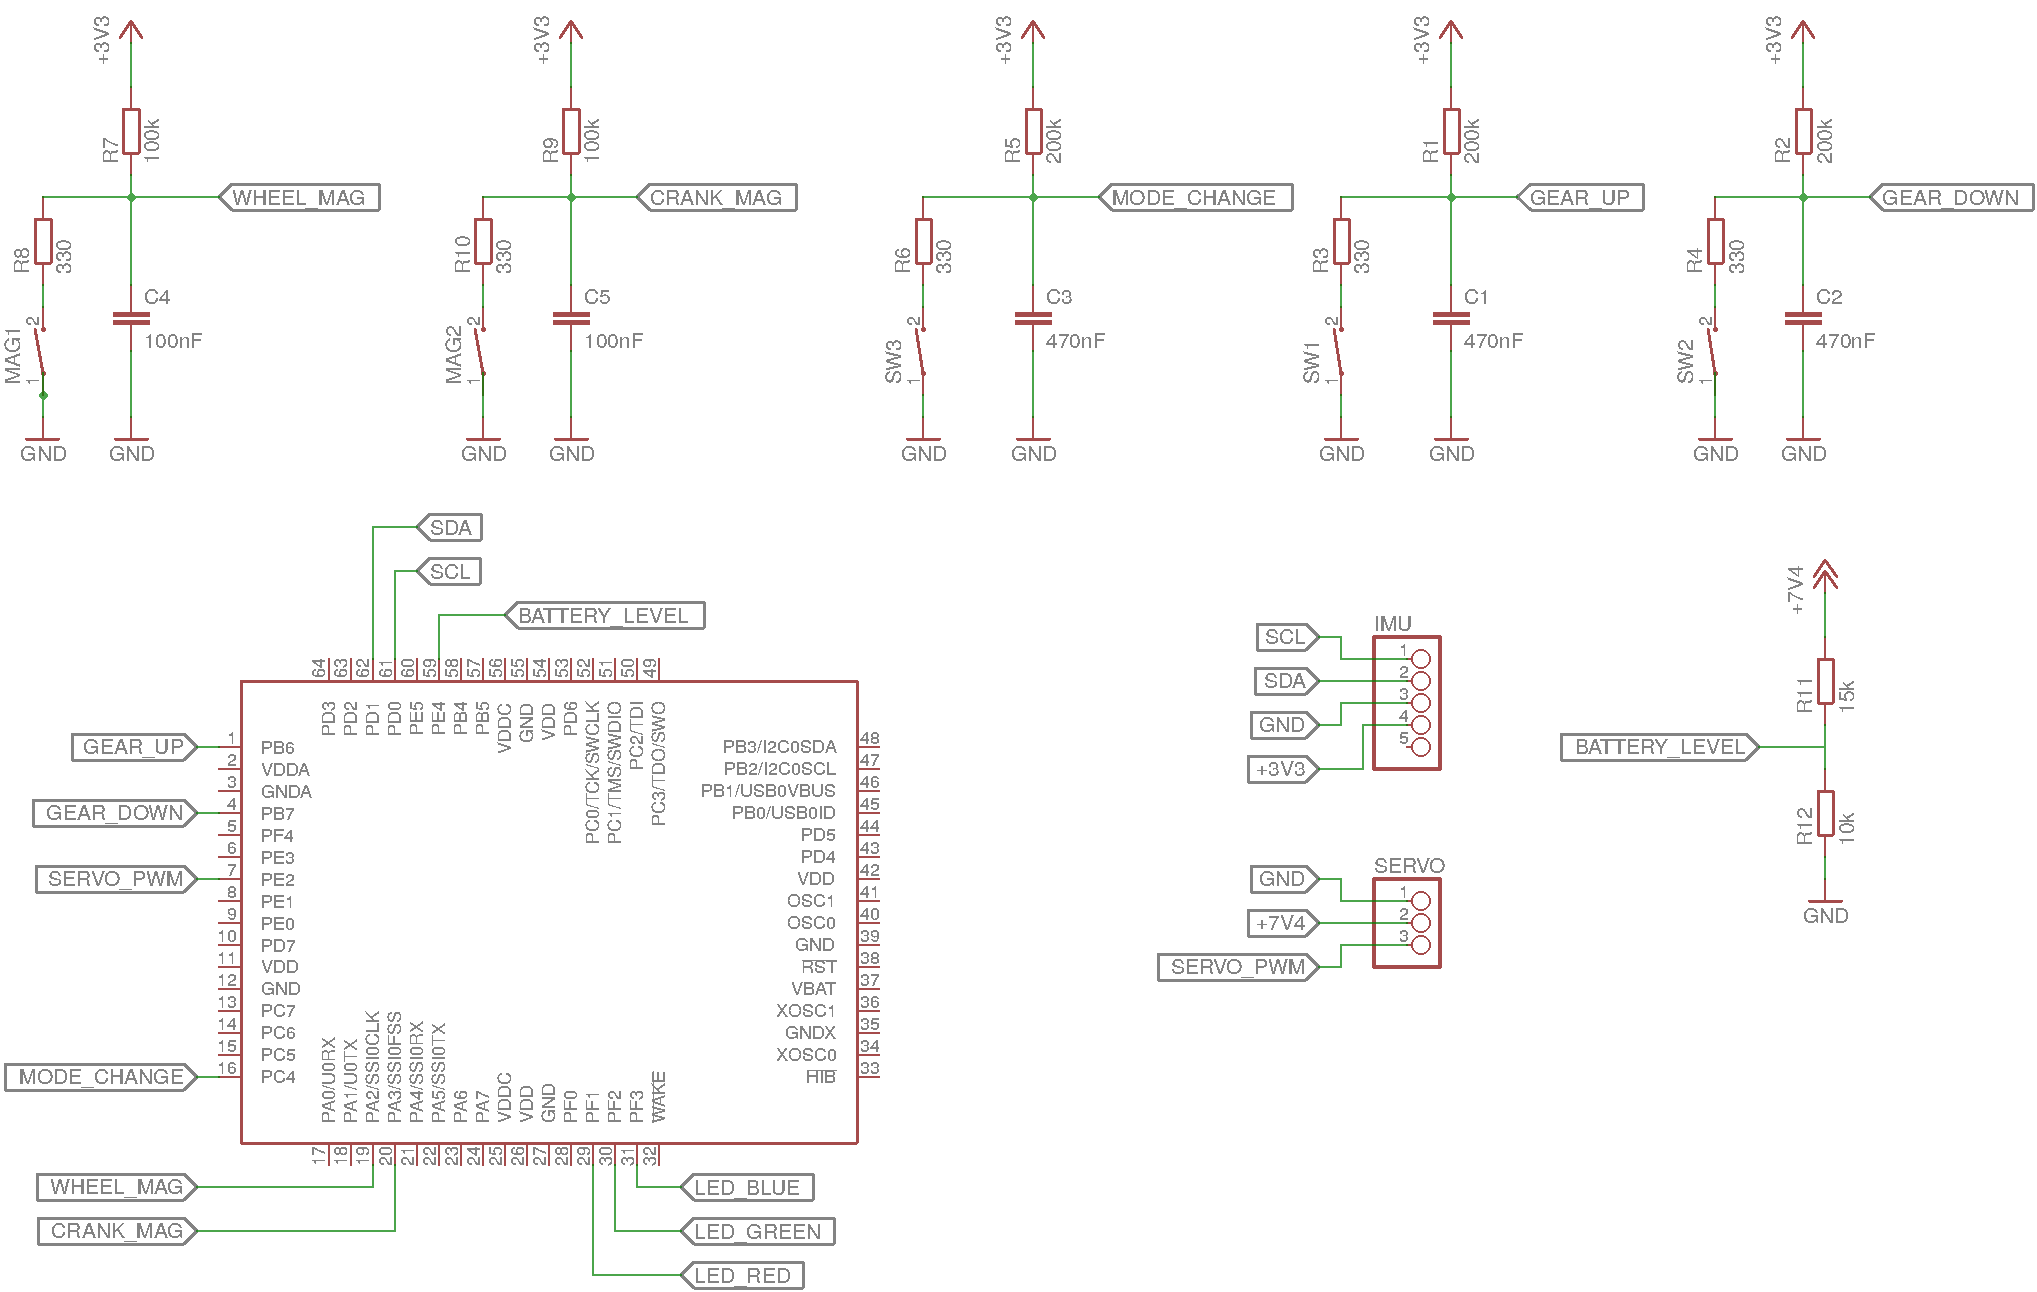
\includegraphics[scale=0.7]{connectionSchematic.png}
    \caption{Schemat ilustrujący zasadę działania programu kontrolera}
    \label{fig:schematPolaczen}
\end{figure}
%_______________________________________________________________________________________________________________

\section{Część programowa}
\subsection{Struktura programu}

Cel pracy to wykonanie układu zmiany przełożeń, który oferuje dwa tryby pracy - tryb ręczny oraz automatyczny. Autor zdecydował, że w ramach trybu automatycznego wykonany zostanie podział na tryb comfort, active i sport. Inspiracją  takiego rozwiązania jest branża motoryzacyjna, w której coraz częściej można spotkać układy automatycznej zmiany przełożeń, oferujące możliwość profilowania charakterystyki działania zmiany biegów, poprzez wybór jednego z trybów jazdy. 

Zasada działania programu przedstawiona zotała na rys. \ref{fig:schematAlgorytmu} i może zotać porównana do skończonej maszyny stanów. Maszyna stanów jest pojęciem abstrakcyjnym, które definiuje zachowanie systemu jako skończony zbóir stanów oraz przejść pomiędzy stanami. Autor rozważał wykorzystanie systemu czasu rzeczywistego \textit{freeRTOS}, w którym poszczególne stany będą odpowiadały nowym zadaniom, odpalanym sekwencyjnie. Jednak właśnie ze względu na sekwencyjne wykonywanie głównych zadań oraz brak ostrych wymagań czasowych, pomysł ten został odrzucony. Program działa na prostej zasadzie pętli nieskończonej, w której poszczególne zadania wyzwalane są przez układy czasowo-licznikowe. Dlatego porównanie programu do skończonej maszyny stanów odnisi się jedynie do wysokopoziomowego opisu zasady działania kontrolera. 

Cztery stany odpowiadają zaprojektowanym trybom jady - tryb ręczny, comfort, active oraz sport. Przejścia pomiędzy tymi stanami następują w wyniku naciśnięcia przycisku zmiany aktualnego trybu jazdy. Kolejność przejść przedstawiona została na rys. \ref{fig:schematAlgorytmu}. Wyróżnione zostały również trzy stany alarmowe - błąd komunikacji I2C, niski poziom naładowania pakietu zasilającego i rozładowanie pakietu zasilającego. 
\begin{figure}[h]
    \centering
    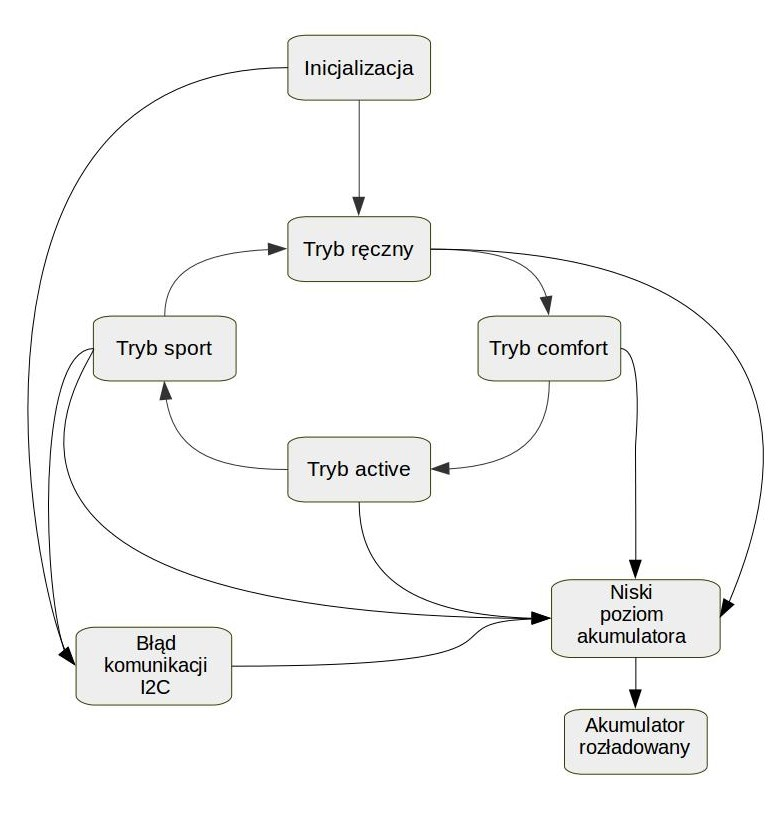
\includegraphics[scale=0.42]{schematAlgorytmu.jpg}
    \caption{Schemat ilustrujący zasadę działania programu kontrolera}
    \label{fig:schematAlgorytmu}
\end{figure}
\subsubsection{Inicjalizacja peryferiów}
Stan inicjalizacji jest stanem początkowym programu, osiąganym jednokrotnie po włączeniu zasilania. W tym stanie następuje inicjalizacja wszystkich układów peryferyjnych. 

Inicjalizowane są:
\begin{itemize}
\item
Porty wejściowe odpowiedzialne za obsługę przycisków do zmiany przełożeń oraz czujników magnetycznych.
\item
Porty wyjściowe odpowiedzialne za generowanie sygnału sterującego serwomechanizmem oraz sterowanie wstaźnikiem RGB aktualnego stanu programu. 
\item
Inercyjna jednostka pomiarowa
\item
Układy czasowo licznikowe, które inicjują zadania okresowe oraz wykorzystywane są do pomiaru prędkości obrotowej i kadencji
\end{itemize}

W przypadku, gdy inicjalizacja wszystkich układów przebiegnie bez błędów, następuje przejście do nastepnego stanu - tryb ręczny.
\subsubsection{Tryb ręczny}
Tryb ręczny jest pierwszym stanem, w którym użytkownik może korzystać z funkcjonalności układu zmiany przełożeń. Zasada działania odpowiada w pełni mechanicznemu układowi. W tym trybie obsługiwane są jedynie przyciski do zmiany przełożeń. Oprogramowanie umożliwia jednokrotną zmianę przełożenia, aktywowaną poprzez naciśnięcie odpowiedniego przycisku. Dodatkowo zaimplementowana została ciągła zmiana przełożeń, która uruchamiana jest poprzez naciśnięcie i przytrzymanie odpowiedniego przycisku. Przełożenia zmieniane są co 1 sekundę, więc użytkownik ma odpowiedniu dużo czasu do zatrzymania zmiany na odpowiednim przełożeniu.

Naciśnięcie przycisku zmiany trybu pracy układu powoduje przejście do kolejnego stanu - trybu comfort.

\subsubsection{Tryb comfort}
Stan comfort odpowiada pierwszemu z zaimplementowanych trybów automatycznej zmiany przełożeń. Ten tryb jest przeznaczony do spokojnego przemieszczania się na rowerze po płaskim terenie. Jest to najprostszy z trybów automatycznych, w którym użytkownik nie powinien angażować się w podejmowanie wyboru przełożenia. Możliwość zmiany ręcznej jest wyłączona. Mierzona jest jedynie chwilowa wartość kadencji. Płaski charakter trasy sprawia, że cykliczne zadanie, w trakcie którego dobierane jest przełożenie, zależne od wartości kadencji, uruchamiane jest z niską częstotliwością. Zakres kadencji jest stały dla każdego przełożenia i dobrany w taki sposób, aby umożliwić spokojną i komfortową jazdę na rowerze. W trakcie przejazdów testowych Autor stwierdził, iż jazda komfortowa odpowiada utrzymaniu kadencji w zakresie od $45$ do $60$ obrotów na minutę.
%_____________________________________________________________________________________________________________
\subsubsection{Tryb active}
Stan active odpowiada drugiem z zaimplementowanych trybów automatycznej zmiany przełożeń. Autor założył, iż ten tryb powinien być używany na trasach o zróżnicowanej topografii terenu. Dlatego zadanie cykliczne dla tego trybu uruchamiane jest z większa częstotliwością, niż w przypadku trybu comfort - raz na dwie sekundy. Zakres kadencji jest stały dla każdego przełożenia. Ze względu na zmienną topografię terenu, został rozszerzony względem trybu comfort i wynosi od $45$ do $70$ obrotów na minutę. Możliwa jest również ręczna zmiana przełożeń, która wskazuje na chęć przęjęcia kontroli nad przełożeniami przez użytkownika. W takiej sytuacji zadanie cykliczne wyłączane jest na $10$ sekund. W tym czasie kontroler nie ma wpływu na dobór przełożeń. W tym trybie brana pod uwagę jest również chwilowa wartość prędkość roweru. Jeśli zostanie wykryty brak obrotów mechanizmu korbowego, następuje automatyczny dobór przełożenia, zgodny z tabelą \textcolor{red}{tabelaprzelozen}, które zostanie ustawione w momencie wznowienia pedałowania. Ma to na celu umożliwienie zmiany o kilka przełożeń w przypadku, gdy rozpoczął się zjazd, a użytkownik przerwał pedałowanie. Ponowne wznowienie pedałowania skutkuje natychmiastowym doborem przełożenia dostosowanym do aktualnej prędkości, bez potrzeby przechodzenia przez poszczególne biegi. 
%_____________________________________________________________________________________________________________

\subsubsection{Tryb sport}  
Stan sport odpowiada ostatniemu z zaimpelementowanych trybów automatycznej zaminy przełożeń. Tryb ten powinien być używany w trakcie bardzo dynamicznej jazdy na rowerze, której celem jest przejechanie danej trasy w jak najkrótszym czasie. Zadanie cykliczne tego trybu jazdy uruchamianje jest z taką samą częstotliwością, jak w przypadku trybu active. Autor podjął taką decyzję, ponieważ uważa, iż częstsze zmiany przełożeń w rowerze są nieefektywne. Zamiast skupić się na generowaniu mocy, użytkownik skupia się na szybkiej pracy układu zmiany przełożeń. Tak jak w trybie active, możliwa jest ręczna zmiana przełożeń, która implikuje wyłączenie kontrolera na $10$ sekund. Przełożenia dobierane są w zależności od wartości kadencji. W przeciwieństwie do pozostałych trybów, zakresy kadencji nie są stałe. Uzależnione zostały od poziomu kąta nachylenia trasy rowerowej. Rozróżniane są 3 możliwości:
\begin{itemize}
\item
Nachylenie terenu jest mniejsze niż $-3^{\circ}$. Oznacza to zjazd ze zbocza o nachyleniu większym, bądź równym $5\%$. Zakres kadencji jest obniżony względem jazdy po płaskim terenie i wynosi \textcolor{red}{ostatecznaWartosc}
\item
    Nachylenie terenu jest należy do zakresu od $-3^{\circ}$ do $3^{\circ}$. Oznacza to jazdę po płaskim terenie. Zakres kadencji taki, jak w trybie active.
\item
Nachylenie terenu jest większe niż $3^{\circ}$. Oznacza to podjazd pod zbocze o nachyleniu większym bądź równym $5\%$. Zakres kadencji jest podwyższony względem jazdy po płaskim terenie i wynosi \textcolor{red}{zakresfinalny}

\end{itemize}
%______________________________________________________________________________________________________________
\subsubsection{Błąd komunikacji I2C}
Przejście do tego stanu może nastąpić w dwóch przypadkach. Pierwszy z nich to problemy z komunikacją w trakcie inicjalizacji jednostki pomiarowej wynikające z braku fizycznego połączenia pomiędzy jednostką pomiarową a portami mikrokontrolera. Drugi to problemy związane z odczytem danych w trybie sport. W tym przypadku może również dojść do problemów z komunikacją. Druga przyczyną mogą być niepoprawne wartości zwracane przez czujniki, świadczące o ich uszkodzeniu.

Problemy z komunikacją objawiają się brakiem odpowiedzi jednostki pomiarowej na rozkazy wysyłane przez mikrokontroler. Przed każdą próbą komunikajci odpalany jest układ czasowo-licznikowy. Jeśli odpowiedź od jednostki przyjdzie w krótszym czasie, niż jedna sekunda po wysłaniu zapytania, układ mierzący czas jest wyłączany. W przeciwnym przyadku wykryty zostaje błąd komunikacji.  
%_____________________________________________________________________________________________________________
\subsubsection{Niski poziom oraz rozładowanie pakietu}

Obydwa stany odnoszą się do problemu z pakietem zasilającym. Niski poziom naładowania odnotowywany jest wtedy, gdy napęcie pakietu zasilającego spadnie poniżej $6.8V$. Następuje wtedy ograniczenie funkcjonalności systemu w ceu oszczędności energii. Program przechodzi do stanu ręcznej zmiany przełożeń. Tryby automatycznej zmiany zostają wyłączone. W efekcie nie są obsługiwane żadne czujniki pomiarowe.

Jeśli napięcie pakietu zasilającego spadnie poniżej $6V$, kontroler przechodzi w tryb pracy z rozładowanym pakietem zasilającym. Jest to tryb maksymalnej oszczędności energii. Wyłączona zostaje możliwość zmiany przełożeń. Działa jedynie dioda RGB sygnalizująca rozładowanie pakietu.

Autor zakłada, że następstwem osiągnięcia tych stanów jest naładowanie pakietu zasilającego. Nie ma zatem możliwości powrotu z tych stanów do normalnej pracy układu. Tak samo dzieje się w przypadku problemów z jednostką pomiarową.
\label{niskiPoziom}
%______________________________________________________________________________________________________________
\subsection{Wskaźnik aktualnego trybu}
Wskaźnik aktualnego stanu, w którym znajduje się kontroler, jest istotnym elementem układu. Umożliwia  użytkownikowi sprawdzenie aktualnego trybu jazdy oraz informuje o stanach alaromowych. Autor uznał, iż dobrym wskaźnikiem aktualnego stanu będzie dioda RGB, która pozwala na zakodowanie wszystkich stanów w postaci odpowiednich kolorów. Taka reprezentacja stanów, w porównaniu np. do wyświetlacza, wydaje sie być bardziej efektywna w trudnym terenie, gdzie rower narażony jest na duże wstrząsy i odczyt z ekrany mógłby zabrać więcej czasu. Do tego montaż prostej diody w okolicy kierownicy jest zdecydowanie prostszy i mniej narażony na uszkodzenia.
Kodowanie stanów w postaci kolorów diody RGB przedstawione zostało w tabeli \ref{tab:rgb}
\begin{table}[h]
    \caption{Pozycja serwomechanizmu oraz czas wypełnienia sygnału PWM w zależności od aktualnego przełożenia.}
    \begin{center}
		\label{tab:rgb}
		\begin{tabular}{|c|c|}
			\hline
 			\textbf{Stan programu} & \textbf{Kolor RGB}\\
 			\hline
 			Inicjalizacja & biały\\  
 			\hline
			Tryb ręczny & żółty\\
			\hline
			Tryb comfort & zielony \\  
			\hline
			Tryb active & niebieski\\  
			\hline
			Tryb sport & różowy \\  
			\hline
			Niski poziom naładowania pakietu & czerwony migający\\  
			\hline
			Pakiet rozładowany & czerwony \\  
			\hline
			Błąd komunikacji I2C & biały migający\\  
			\hline
		\end{tabular}
	\end{center}
\end{table}

%______________________________________________________________________________________________________________

\section{Szczegóły implementacji}
%_______________________________________________________________________________________________________________
\subsection{Kontrola serwomechanizmu}
Pozycja serwomechanizmu modelarskiego sterowana jest przez sygnał PWM (z ang. {\em Pulse-Width Modulation}). Jest to metoda regulacji sygnałem napięciowym, o stałej częstotliwości i amplitudzie, polegająca na zmianie wypełnienia sygnału. Częstotliwość sygnału wynosi 50Hz. Wartości napęcia, które zmianiają się w sposób skokowy, wynoszą 0 i 3.3V. Pełny zakres ruchu serwomechanizmu osiągalny jest przez zmianę wypełnienia sygnału sterującego z zkresu od 2.5 do 12.5 \%. Innymi słowy - podanie prostokątnego sygnału sterującego o okresie 20ms, w którym stan wysoki utrzymany jest przez czas z zakresu od 0.5ms do 2.5 ms, umożliwia obrót wału serwomechanizmu z zakresu od 0 do 180$^{\circ}$.

Przerzutka, do której został przymocowany serwomechaznim, ogranicza pełny zakres ruchu serwomechanizmu. Minimalne oraz maksymalne wychylenie wózka przerzutki wiąże się z obrotem wału serwomechanizmu odpowiednio o kąt 31 i 95$^{\circ}$. W tym zakresie obsługiwane sa wszystkie dostępne przełożenia. Każdemu z ośmiu przełożeń odpowiada inna pozycja serwomechanizmu (tabela \ref{tab:przelozenia}). Pozycje serwomechanizmu zostały dobrane eksperymentalnie. Można zaobserwować liniowy przyrost czasu wypełnienia sygnału. 
\begin{table}[h]
    \caption{Pozycja serwomechanizmu oraz czas wypełnienia sygnału PWM w zależności od aktualnego przełożenia.}
    \begin{center}
		\label{tab:przelozenia}
		\begin{tabular}{|m{2.3cm}|m{3cm}|m{3cm}|}
			\hline
 			Nr przełożenia & Pozycja serwomechanizmu [$^{\circ}$] & Czas wypełnienia sygnału [$us$] \\
 			\hline
 			1 & 31.5 & 850 \\  
			2 & 40.5 & 950 \\
			3 & 49.5 & 1050 \\  
			4 & 58.5 & 1150 \\  
			5 & 67.5 & 1250 \\  
			6 & 76.5 & 1350 \\  
			7 & 85.5 & 1450 \\  
			8 & 94.5 & 1550 \\  
			\hline
		\end{tabular}
	\end{center}
\end{table}

Z doświadczenia autora pracy wynika, że zmiana przełożeń w konwencjonalynch układach napędowych działa znacznie lepiej, jeśli w trakcie zmiany beigu następuje chwilowe przeciągnięcie pozycji wózka przerzutki. Jest to szczególnie dobrze widoczne w trakcie redukowania przełożenia, kiedy łańcuch powinien trafić na koło zębate o większej średnicy. Można wtedy zaobserwować opóźnienie w zmianie przełożenia, niekorzystne przeskoki łańcucha pomiędzy kołami zębatymi, a w źle wyregulowanych układach napędowych może nawet dochodzić do braku reakcji układu napędowego. Takie zjawisko zostało zaobserwowane w trakcie pracy nad projektem. Zmiana biegów polegająca na pozycjonowaniu serwomechanizmu w nowej pozycji, zależnej od dobranego przełożenia, działała z wyraźnym opóźnieniem. Problem, podobnie jak w układach mechanicznych, został rozwiązany przez chwilowe przeciągnięcie pozycji wózka przerzutki. Zdefiniowanie zostały dwa pomocnicze zestawy pozycji serwomechanizmu, specyficzne dla redukowania oraz zwiększania przełożenia(tabela \ref{tab:przelozeniaPomocniczne}). Wszystkie trzy zestawy pozycji przechowywane są w postaci tablic, które zawierają czasy wypełnienia sygnału sterującego. W momencie rozpoczęcia zmiany przełożenia, na skutek naciśnięcia przycisku lub w wyniku decyzji kontrolera automatycznej zmiany przełożeń, zmienna, która do tej pory wskazywała na główny zestaw pozycji, zaczyna wskazywać na jeden z zestawów pomocniczych zależny od rodzaju zmiany. Jednocześnie uruchominy zostaje układ czasowo-licznikowy. Po upływie 500ms, w trakcie obsługi przerwania tego układu, następuje przypisanie adresu, pod którym znajduje się w pamięci główny zestaw parametrów. Następuje również wyłączenie układu czasowo-licznikowego. 


\begin{table}[h]
    \caption{Pomocnicze zestawy pozycji serwomechanizmu}
    \begin{center}
		\label{tab:przelozeniaPomocniczne}
		\begin{tabular}{|p{2.3cm}|p{5cm}|p{5cm}|}
			\hline
 			Nr przełożenia & Wypełnienie sygnału w trakcie redukcji przełożenia [$us$] & 
Wypełnienie sygnału w trakcie zwiększenia przełożenia [$us$] \\
 			\hline
 			1 & 800 & 900 \\  
			2 & 900 & 1000 \\
			3 & 1000 & 1100 \\  
			4 & 1100 & 1200 \\  
			5 & 1200 & 1300 \\  
			6 & 1300 & 1400 \\  
			7 & 1400 & 1500 \\  
			8 & 1500 & 1600 \\  
			\hline
		\end{tabular}
	\end{center}
\end{table}
%______________________________________________________________________________________________________________
\subsection{Obsługa przycisków}
W projekcie wykorzystane zostały trzy przyciski przewlekane monostabilne. Ich naciśnięcie powoduje redukcję lub zwiększenie przełożenia oraz zmianę trybu pracy kontrolera. Przyciski do zmiany przełożenia zamontowane zostały w miejscu konwencjonalnej manetki. Przycisk do zmiany trybu pracy został przymocowany do mosktka kierownicy.

Wszystkie przyciski wykorzystują rezystor pull-up, podciągający do portu wejściowego napięcie 3.3V(rys. \ref{fig:schematPolaczen}). Zwarcie przycisku powoduje ustalenie sygnału na poziomie 0V. Pojawienie się na magistrali zbocza opadającego powoduje zgłoszenie przerwania od odpowiedniego pinu portu wejściowego. 

Z przyciskami związany jest problem drgań styków w trakcie zwierania/rozwiearania przycisku. Są to drgania mechaniczne, które moga trwać od kilku mikrosekund do nawet kilkunastu milisekund. Powoduje to niezdefiniowane zachowanie całego systemu, np. zmianę kilku przełożeń na raz. Szybkozmienne zmiany stanu logicznego sygnału, wynikające z drgań sytków przycisku, przedstawione zostały na rys \ref{fig:drganiaPrzyciskow}.
\begin{figure}[h]
    \centering
    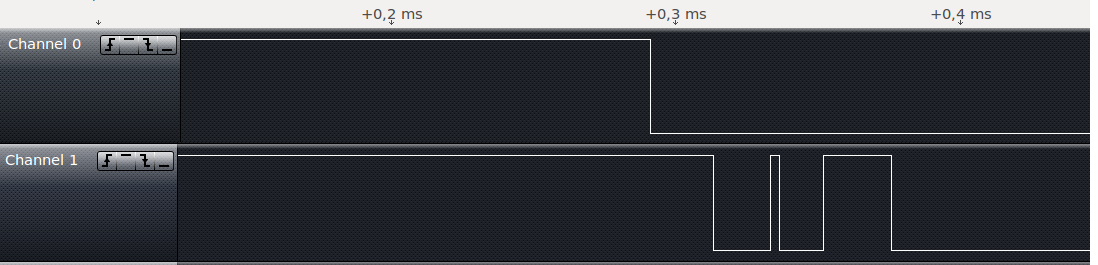
\includegraphics[scale=0.2]{drganiaPrzyciskow.png}
    \caption{Porównanie przebiegów sygnałów interpretowanych przez analizator stanów logicznych dla przycisku z filtrem RC - kanał 0, oraz bez filtra- kanał 1.}
    \label{fig:drganiaPrzyciskow}
\end{figure}
Istnieje kilka sposobów rozwiązania tego problemu. Można je podzielić na sposoby programowe oraz sprzętowe. Sposoby programowe to np. kilkukrotne sprawdzenie stanu portu wejściowego lub chwilowe wyłączenie przerwań od portów wejściowych. Autor zdecydował, że lepszym rozwiązaniem będzie usunięcie przyczyny tego zjawiska, czyli odpowiednie kondycjonowanie sygnału. W tym celu wykoanne zostały proste filtry dolnoprzepustowe RC. Zasada działania filtru RC została opisana w pkt. \ref{filtrRc}. W dokumentacji mikrokontrolera(\textcolor{red}{link}) można znaleźć informację na temat minimalnego poziomu napięcia, interpretowanego jako stan wysoki - $0.6V_{in}$. Podobny poziom napięcia osiągany jest na wyjściu filtru RC, po skokowej zmianie napięcia wejściowego, po czasie równym stałej czasowej filtra. Autor założył, że zmiany biegów, oraz zmiana tryb jazdy, nie mogą być dokonywane częciej, niż 10 razy na sekundę. Z tego wynika, że stała czasowa filtru powinna wynosić około $100ms$. Wszystkie 3 filtry zostały wykonane w oparciu o opornik o rezystancji $200k\Omega$ i kondensator o pojemności 470$nF$. Tak dobór elementów pasywnych pozwala zbudować filtr, którego stała czasowa wynosi około $94ms$ 
%______________________________________________________________________________________________________________
\subsection{Kontrola zbliżeniowych czujników magnetycznych}
Zbliżeniowe czujniki magnetyczne działają w sposób analogiczny do przycisków monostablilnych. Różnica polega na tym, że styki zwierane są w wyniku działania zewnętrznego pola magnetycznego, pochodzącego od magnesu trwałego. W trakcie zwierania/rozwierania czujnika magnetycznego również pojwia się problem mechanicznych grań styków. Problem został wyeliminowany w taki sam sposób, jak w przypadku przycisków, czyli przez zastosowanie filtrów dolnoprzepustówych RC. Elementy pasywne filtrów RC Stałe dla czujników magnetycznych zostały dobrane zgodnie z poniższymi założeniami.

Czujnik magnetyczny, wykorzystany do wyznaczania chwilowej wartości prędkości roweru, korzysta z dwóch magnesów trwałych. Doświadczenia przeprowadzone z wykorzystaniem analizatora stanów logicznych przy dużych prędkościach obrotowych tylego koła wykazały, że drgania czujników magnetycznych trwają nie dłużej niż $1ms$.  Autor założył, że maksymalna prędkość roweru możliwa do osiągnięcia to $100\frac{km}{h}$, czyli około $28\frac{m}{s}$. Promień koła roweru wynosi około $0.33m$. Z zależności \ref{eq:zaleznoscNaPredkosc} wynika, że dla prędkości maksymalnej, magnes trwały znajduje się w pobliżu czujnika magnetycznego co $37ms$. Należy uwzględnić również to, że w tym czasie dochodzi do zwarcia i rozwarcia czujnika magnetycznego. Stała czasowa filtru RC, powinna być zatem co njamniej dwa razy krótsza. Ostatecznie filtr RC został wykonany z opornika o rezystancji $100k\Omega$ i kondensatora o pojemności $100nF$, co zapewnia wartość stałej czasowej filtra na poziomie $10ms$. Wartość ta jest o rząd wielkości większa od zarejestrowanych okresów drgań, a jednocześnie zwarcie i rozwarcie czujnika z filtrem trwa prawie dwa razy krócej, niż okres obrotu magnesu trwałego dla przyjętej prędkości maksymalnej.

Czujnik magnetyczny wykorzystywany do wyznaczenia chwilowej wartości kadencji jest zwierany przez jeden magnes trwały, przymocowany do ramienia mechanizmu korbowego. Autor przyjął, że maksymalna kadencja możliwa do osiągnięcia przez rowerzystę, to $250\frac{obr}{min}$. Pełny obrót przy takie kadencji zajmuje $240ms$. Zastosowanie filtru o takej samej stałej czasowej, jak filtr czujnika magnetycznego prędkości roweru, spełnia wymagania wynikające z przyjętego założenia o maksymalnej kadencji. 
%______________________________________________________________________________________________________________
\subsection{Obsługa jednostki pomiarowej Pololu AltIMU10}
Dane pomiarowe pochodzące z akcelerometru oraz żyroskopu wykorzystywane są w trybie active i sport. Kąt nachylenia podłoża wyznaczany jest co $10ms$ przy użyciu filtru komplementarnego (pkt. \ref{kompZasadaDzialania}). 
 
Komunikacja pomiędzy mikrokontrolerem a jednostką pomiarową zachodzi przy użyciu magistrali I2C. Magistrala działa w tybie \textit{standard mode}, w którym prędkość transmisji danych wynosi $100kb/s$. Jednostka pomiarowa posiada pięć pinów wyjściowych, jednak używane są tylko cztery:
\begin{itemize}
    \item
    SCL(z ang. {\em Serial Clock Line}) - linia zergarowa wykorzystana do synchronizacji transferu danych
    \item
    SDA(z ang. {\em Serial Data Line}) - linia danych wykorzystana do transferu danych
    \item
    Vin - zasilanie jednoski pomiarowej, które przyjmuje napięce z zakresu od 2.5V do 5.5V
    \item
    Gnd - wspólna masa
\end{itemize} 

Komunikacja w standardzie I2C jest komunikacją typu master/slave. Urządzeniem nadrzędnym, odpowiedzialnym za inicjowanie, prowadzenie oraz kontrolę transmisji, jest mikrokontroler. Urządzenia pomiarowe to urządzenia typu slave. Każdy z układów pomiarowych posiada swój unikalny, 7-bitowy adres. Każde z urządzeń typu slave udziela odpowiedzi na rozkazy wysyłane przez mikrokontroler. Adresy urządzeń jednostki pomiarowej:

\begin{table}[h]
    \caption{Adresy urządzeń pomiarowych}
    \begin{center}
		\label{tab:adresyImu}
		\begin{tabular}{|c|c|}
			\hline
 			Urządzenie & Adres \\
 			\hline
 			Akcelerometr & 0x19 \\  
 			\hline
			Żyroskop & 0x6B \\
			\hline
			Magnetometr & 0x1E \\  
			\hline
		\end{tabular}
	\end{center}
\end{table}

Biblioteka TivaWare udostępnia metody do obsługi komunikacji I2C. Akcelerometr został skonfigurowany w taki sposób, aby obsługiwał zakres przyspieszeń $\pm2g$. Żyroskop obsługuje zakres pomiarowy $\pm245dps$.
%______________________________________________________________________________________________________________
\subsection{Pomiar poziomu naładowania pakietu zasilającego}

Układ do pomiaru poziomu baładowania baterii został zbudowany w oparciu o przetwornik analogowo-cyfrowy oraz dzielnik napięcia. 

Napięcie robocze pojedynczego ogniwa li-po wynosi 3.4V. W trakcie pracy ogniwa napięcie może się wahać - od 3.0V w przypadku rozładowania, do nawet 4.2V zaraz po naładowaniu ogniwa. Pakiet zasilający układu składa się z dwóch ogniw li-po, zatem napięcie może przyjmować wartości od 6V do 8.8V. Pomiar tej wielkości przez przetwornik analogowo-cyfrowy nie jest możliwy, gdyż przekracza maksymalne dopuszczalne napięcie na porcie wejściowym mikrokontrolera, które wynosi 5.5V(\textcolor{red}{datasheet, str 1360}). W celu obniżenia napięcia zastosowany został dzielnik napięcia. Dzielnik napięcia to czwórnik, który pozwala zapewnić odpowiedni stosunek pomiędzy napięciem wejściowym a napięciem wyjściowym układu. Napięciem wejściowym układu jest napięcie pakietu zasilającego, a napięciem wyjściowym jest napięcie podane na przetwornik analogowo-cyfrowy, tak jak zostało to przedstawione na rys. \ref{fig:schematPolaczen}.
\begin{figure}
    \centering
    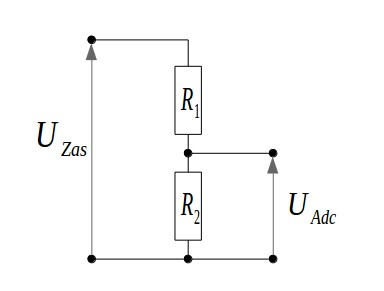
\includegraphics[scale=0.5]{dzielnikNapiecia.jpg}
    \caption{a nice plot}
    \label{fig:równia}
\end{figure}

Napięcie na wyjściu dzielnika napięcia określone jest zależnością:
\begin{equation}
    U_{Adc}=U_{Zas}\frac{R_2}{R_1 + R_2}
    \label{eq:rownanieDzielnik}
\end{equation}

Zakładając maksymalną wartość napięcia pakietu, napięcie wejściowe na przetworniku analogowo-cyfrowym powinno wynosic 3.3V a rezystancja $R_2$ jest równa $10k\Omega$, to zgodnie z zależnością \ref{eq:rownanieDzielnik} rezystancja $R_1$ powinna przyjąć około $15k\Omega$.

Przetwornik analogowo-cyfrowy przetwarza sygnał analogowy na równoważną postać cyfrową. Mikrokontroler wyposażony jest w przetwornik 12-bitowy. Oznacza to, że do reprezentacji całego zakresu pomiarowego używa dwunastu bitów. Zakres pomiarowy określony jest przez sygnały referencyjne - $0V$ i $3.3V$(\textcolor{red}{datasheet808}). Wartość zwracana przez przetwornik dla napięcia $0V$ wynosi $0$, natomiast dla napięcia $3.3V$ przetwornik zwraca liczbę $4096$. Rozdzielczość przetwornika wynosi około $0.8mV$

Zgodnie z pkt. \ref{niskiPoziom}, zgłaszane są dwa stany alarmowe związane z zasilaniem:
\begin{itemize}
\item
    stan niskiego poziomu naładowania pakietu zasilającego wynoszący 6.8V
\item
    stan rozładowania pakietu zasilacjącego wynoszący 6V.
\end{itemize}

Biorąc pod uwage powyższe zależności oraz założenia, można wyznaczyć wartości zwracane przez przetwornik dla stanów alarmowych - tabela \ref{tab:napieciaDwojnik}

\begin{table}[h]
    \caption{Poziomy napięć alarmowych oraz wartości zwracane przez przetwornik}
    \begin{center}
		\label{tab:napieciaDwojnik}
		\begin{tabular}{|c|c|c|}
			\hline
 			Napięcie $U_{Zas}$ [V]& Napięcie $U_{Adc}$ [V]& Wartość zwracana przez przetwornik \\
 			\hline
 			6.8 & 2.72 & 3376 \\  
 			\hline
			6.0 & 2.4 & 2979 \\
			\hline
		\end{tabular}
	\end{center}
\end{table}




